\section{The physics of interacting wave}

\subsection{Dispersive PDEs}\label{sec.dispintro}
In this thesis, we will mostly be interested in the long time behavior of dispersive PDEs on a finite domain.
\begin{equation}
    i\partial_t \phi = \Lambda(\nabla) \phi + \lambda B(\phi,\phi)\ (\text{or } \lambda^2 C(\phi,\phi,\phi))
\end{equation}

Examples of equations of the above type are listed below.
\begin{enumerate}
    \item The nonlinear Schrodinger equations
    \begin{equation}\label{eq.NLS}
        i\partial_t\psi-\Delta\psi=\pm\lambda^2 |\psi|^2\psi
    \end{equation}
    \item The ZK equation
    \begin{equation}\label{eq.ZK}
        \partial_t\psi(t,x)+\Delta\partial_{x_1}\psi(t,x)-\nu \Delta \psi(t,x)=\lambda \partial_{x_1}(\psi^2(t,x))
    \end{equation}
    \item The nonlinear Klein-Gordon equation
    \begin{equation}\label{eq.KG}
        \partial_{tt}u-\Delta u=\pm\lambda^2 u^3 \ (\text{or } u^2)
    \end{equation}
    \item The rotating Navier-Stokes equation (we only give the incompressible equation)
    \begin{equation}\label{eq.rNS}
        \left\{
        \begin{aligned}
            &\partial_t u + u\cdot \nabla u + e_z\times u + \nabla p = \nu \Delta u,
            \\
            & \text{div}\, u = 0.
        \end{aligned}\right.
    \end{equation}
    \item Internal wave in the stratified fluid
    \begin{equation}\label{eq.SF}
        \left\{
        \begin{aligned}
            &\partial_t u + u\cdot \nabla u + \frac{1}{\rho}\nabla p = \frac{\nu}{\rho} \Delta u,
            \\
            & \partial_t\rho +u\cdot\nabla\rho = 0
            \\
            & \text{div}\, u = 0.
        \end{aligned}\right.
    \end{equation}
    \item The MHD equation
    \begin{equation}\label{eq.MHD}
        \left\{
        \begin{aligned}
            &\partial_t u + u\cdot \nabla u + \nabla p = b\cdot\nabla b + \nu \Delta u,
            \\
            & \partial_t b + u\cdot \nabla b  = b\cdot\nabla u + \eta \Delta b,
            \\
            & \text{div}\, u = 0,\quad \text{div}\, b = 0..
        \end{aligned}\right.
    \end{equation}
    \item The gravity water wave equation (we do not include the equation due to its complication). 
\end{enumerate}

In the rest part of this introduction, we \textbf{take the nonlinear Schrodinger equation as an example} to explain the idea of wave turbulence. 

\subsection{The energy cascade phenomenon}
It is well-known that in many PDEs coming from physics, energy can be transferred from low-frequency Fourier modes to high-frequency modes. We take the nonlinear Schr\"odinger equation as an example to explain this.

Its Fourier coefficients satisfy
\begin{equation}
\dot{\psi}_{k} =  i|k|^2 \psi_k 
 +\frac{i\lambda^2}{L^{2d}} \sum\limits_{\substack{(k_1,k_2,k_3) \in (\mathbb{Z}^d_L)^3 \\ k_1 - k_2 + k_3 = k}} \psi_{k_1} \overline{\psi_{k_2}} \psi_{k_3}
\end{equation}
$\psi_{k_1}$, $\psi_{k_2}$, $\psi_{k_3}$ can "collide" with each other and transfer energy to $\psi_k$. For example, energy can transfer to $\psi_{6}$ in the "collision" of $\psi_{1}$, $\psi_{2}$, $\psi_{3}$.


This can be repeated many times 
\begin{equation}
    \psi_1\rightarrow \psi_2\rightarrow \psi_4\rightarrow \psi_7\rightarrow \cdots \rightarrow \psi_{100} \rightarrow \cdots.
\end{equation}

This process can be repeated many times so that finally the energy can be injected at a very high frequency. 
%(like $1\rightarrow 2\rightarrow 3\rightarrow\cdots\rightarrow 10^4$)
This is called the energy cascade phenomenon. Since it takes many steps to transfer energy to very high modes, the information in the low-frequency modes is lost and high-frequency modes become random and exhibit \textit{universality}. This is very similar to the game, \textit{Galton board}, as illustrated in Figure \ref{fig.Galtonboard}.
Each step of energy transfer is similar to a collision of a ball with a pin. To get to the bottom (the high energy modes), a ball must collide with many pins (there must be many steps of energy transfer). Finally, the distribution of balls (energy) becomes random and universal.  
\begin{figure}[H]
    \centering
    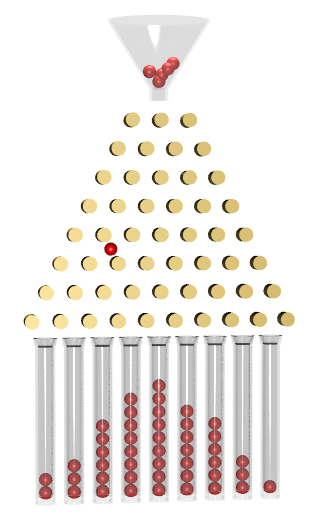
\includegraphics[scale = 0.2]{introduction/Galton_board.png}
    \caption{The Galton board}
    \label{fig.Galtonboard}
\end{figure}

In the Galton board case, the final distribution is the Gaussian distribution. This distribution is universal in the sense that it is independent of the details of the input flow of balls. Although in many examples of energy cascade the final distribution is random and universal, they are usually not i.i.d Gaussian or even do not exhibit properties similar to i.i.d Gaussian.

The cascade spectrum of strong turbulence in the fluid is one example of highly non-Gaussian universality behavior. The structure functions satisfy power laws which are independent of the initial data. The second-order structure function satisfies the famous Kolmogorov $5/3$ law while the high-order structure functions exhibit a significant deviation from Kolmogorov's prediction. This deviation is called \textit{intermittency}. 

\begin{figure}[H]
    \centering
    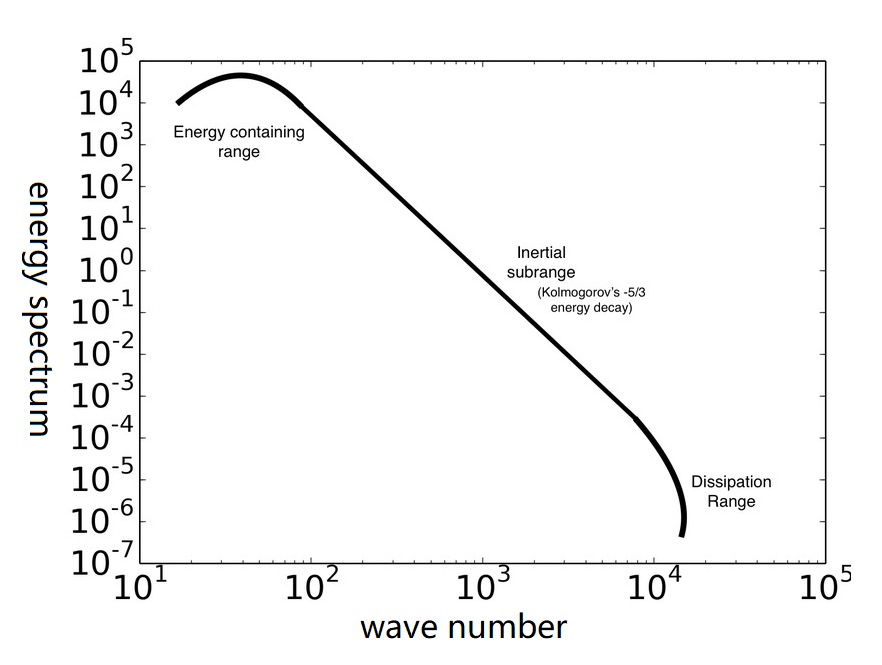
\includegraphics[scale = 0.6] {introduction/five_third_law.png}
    \caption{The $5/3$ law}
    \label{fig.5/3law}
\end{figure}

While i.i.d Gaussian assumption does not work for turbulence in fluid, it can work for turbulence generated by dispersive waves. Unlike a fluid equation, a dispersive equation can exhibit turbulent behavior even when the size of the solution is small. In this case, the distribution can be calculated by a perturbative expansion and it is close to i.i.d Gaussian variables if it is so initially. This kind of turbulence is the so-called \textit{wave turbulence}.


\subsection{The statistical description of interacting wave}

In the study of wave turbulence of the nonlinear Schrodinger equation, we assume that the initial data of the PDE satisfies
\begin{equation}
\psi_{\textrm{in},k}=\sqrt{n_{\textrm{in}}(k)} \eta_k(\omega)
\end{equation}
where $\eta_k(\omega)$ are iid normal complex Gaussian variables.

Then the solution $\psi$ is a random variable. Let $\psi_k$ be its Fourier coefficients, then we define the energy spectral to be $n(t,k)=\mathbb{E}|\psi_k|^2$. The goal of this thesis is to study the evolution of this energy spectral.

For a more general equation, the ansatz of initial data can be imposed similarly. Here is a list of possible modifications,

\begin{enumerate}
    \item If the solution $\psi$ is a complex value function, then the ansatz is the same.
    \item If the solution $\psi$ is a real value function, then to ensure the real value property, we assume that $n_{\textrm{in}}(k)=n_{\textrm{in}}(-k)$, $\eta_k=\overline{\eta_{-k}}$ and $\eta_k$ is independent of $\{\eta_{k'}\}_{k'\ne k,-k}$. 
    \item For second-order equations, we typically introduce a new variable to reduce it into a first-order equation as in section \ref{sec.introfourwave}, and then impose the same ansatz as first-order equations. 
    \item For a system of equations with more than $1$ variable, we assume that the Fourier coefficients of one component are independent of those of another component.
\end{enumerate}

These modifications are not the only canonical choices. The idea of proof of other choices is similar to the above choices.




\subsection{Scale of turbulence}

The energy distribution $n(k)$ looks very different in different ranges. In general, the frequency domain can be divided into 3 parts, the \textit{energy-containing range}, the \textit{inertial range} and the \textit{dissipation range}.

As in Figure \ref{fig.5/3law}, in the energy-containing range $|k|\ll 1$, the wave number $k$ is not large and the energy distribution in this range can be influenced by the external force and initial data. There is no universality in this range. 


In the inertial range $1\lesssim |k|\ll l_d^{-1}$, the same as the Galton's board, the influence of external force and initial data starts to be lost, while the wave number is not large enough to activate the effect of dissipation. The energy distribution is universal and satisfies the \textit{wave kinetic equation} \eqref{eq.WKE} given below.


In the dissipation range $|k|\gtrsim l_d^{-1}$, the effect of dissipation is dominant and $n(k)$ decays to $0$ very fast. In this thesis, we are mostly interested in the energy distribution in the inertial and dissipation range.


In wave turbulence, the energy distribution $n(k)$ is supposed to evolve according to the following wave kinetic equation
\[
\tag{WKE}\label{eq.WKE}
\begin{split}
&\partial_t n(t, k) =\mathcal K\left(n(t, \cdot)\right),
\\
&\mathcal K(n)(k):= \int_{\substack{(k_1, k_2)\in \mathbb{R}^{2d}\\k_1+k_2=k}}\left|H_{k_1k_2}\right|^2n(k_1) n(k_2)\delta(\Lambda(k_1)+\Lambda(k_2)-\Lambda(k))\, dk_1 dk_2
\\
&\text{or }\int_{\substack{(k_1, k_2, k_3)\in \mathbb{R}^{3d}\\k_1-k_2+k_3=k}}\left|H_{k_1k_2k_3}\right|^2n(k_1) n(k_2)n(k_3)\delta(\Lambda(k_1)-\Lambda(k_2)+\Lambda(k_3)-\Lambda(k))\, dk_1 dk_2dk_3
\end{split}
\]
\eqref{eq.WKE} admits a special solution $|k|^{-\nu}$ and the general solution of \eqref{eq.WKE} is supposed to converge to this power law in some regimes. This power law is universal and independent of the detail of external force and initial data.

The \eqref{eq.WKE} is a Boltzmann-type equation. Compared to the original ZK equation, \eqref{eq.WKE} has a monotonically decreasing entropy (see \cite{germain2020optimal}) and exhibits irreversibility. The Boltzmann equation statistically describes the collision of particles and in the collision integral there are momentum and energy conservation conditions $p_1+p_2=p$ and $p^2_1+p^2_2=p^2$. \eqref{eq.WKE} is a counterpart that describes the interaction of waves. The right-hand side of \eqref{eq.WKE} also contains momentum and energy conservation $k_1+k_2=k$,  $\Lambda(k_1)+\Lambda(k_2)=\Lambda(k)$. The energy conservation is the time resonance surface in the space-time resonance method.


\subsection{Three-wave and four-wave models}

For a general dispersive PDE, if the leading order term in the nonlinearity is quadratic and the solution of the resonance surface $\Lambda(k_1)+\Lambda(k_2)=\Lambda(k)$ is non-empty, then we say that this PDE is a \underline{three-wave model}. If the leading order term in the nonlinearity is cubic and the solution of the resonance surface is non-empty, then we say that this PDE is a \underline{four-wave model}. 


In the example of dispersive PDEs in section \ref{sec.dispintro}, the quadratic equations \eqref{eq.ZK}, \eqref{eq.rNS}, \eqref{eq.SF}, \eqref{eq.MHD} are examples of the $3$ wave interaction case. the cubic equations \eqref{eq.NLS}, \eqref{eq.KG} are examples of $4$ wave interaction cases. The quadratic \eqref{eq.KG} equation is a four-wave model because the three wave resonance surface $\sqrt{1+|k_1|^2}+\sqrt{1+|k_2|^2}=\sqrt{1+|k|^2}$ is empty in this case.

In this thesis, we choose the ZK equation as an example of $3$ wave turbulence theory and the Klein-Gordon equation as an example of $4$ wave turbulence theory.  


